\documentclass[a4paper, 10pt, final, garamond]{book}
\usepackage{cours-preambule}
\graphicspath{{./figures/}}

\addto\captionsfrench{\renewcommand{\figurename}{Fig.}}
% \renewcommand{\figurename}{Fig.}

\makeatletter
\renewcommand{\@chapapp}{Contr\^ole de connaissances}
\makeatother

% \toggletrue{student}
\toggletrue{corrige}
\renewcommand{\mycol}{black}
% \renewcommand{\mycol}{gray}

\begin{document}
\setcounter{chapter}{-1}

\settype{enon}
\settype{solu}

\chapter{Rentrée, unités, mesure et optique\ifstudent{~(15')}}

\begin{enumerate}[label=\sqenumi]
	\item[n]{1.5}%
	Citer, sans détailler, les trois astuces pour reprendre le contrôle sur son
	utilisation du téléphone.
	\smallbreak
	\psw{%
		Restriction du temps, contrainte physique et contrainte catégorique.
	}%
	\item[n]{7}%
	Quels sont \textit{a priori} les paramètres pertinents dont dépend la période
	$T$ des oscillations d'un pendule simple~? Déterminer alors, par analyse
	dimensionnelle, son expression. Indiquer une limite de cette technique, puis
	la formule correcte.
	\smallbreak
	\psw{%
		Les variables propres possibles sont $\ell$, $g$ et $m$~; \pt{1} ainsi, il
		nous faudrait avoir
	}%
	\smallbreak
	\noindent
	\begin{isd}
		\psw{%
			\begin{gather*}
				T \stm{=} \ell^{\alpha}g^{\beta}m^{\gamma}
				\\\Lra
				[T] = [\ell]^{\alpha}[g]^{\beta}[m]^{\gamma}
				\\\Lra
				\si{s} \stm[-1]{=} \si{m^{\alpha}.m^{\beta}.s^{-2\beta}.kg^{\gamma}}
				\\\Lra
				\left\{
				\begin{array}{rcl}
					\si{s} & = & \si{s}^{-2 \beta}
					\\
					1      & = & \si{m}^{\alpha+\beta}
					\\
					1      & = & \si{kg}^{\gamma}
				\end{array}
				\right.
				\stm{\Lra}
				\left\{
				\begin{array}{rcl}
					\beta  & = & - \frac{1}{2}
					\\
					\alpha & = & \frac{1}{2}
					\\
					\gamma & = & 0
				\end{array}
				\right.
			\end{gather*}
		}%
		\tcblower
		\psw{%
			Autrement dit, on aurait tendance à écrire
			\[
				\boxed{T \stm{=} \sqrt{\frac{\ell}{g}}}
			\]
			Cependant, cette technique ne permet pas d'obtenir les facteurs
			adimensionnés. \pt{1} L'étude complète du système donne un
			\textbf{facteur}
			$\mathbf{2\pi}$ \pt{1} avant la racine.
		}%
	\end{isd}
	\vspace*{-20pt}
	\item[n]{4}%
	Comment valider une régression linéaire~? Deux éléments sont attendus, ainsi
	que deux schémas grossiers représentatifs de régressions~: une valide et une
	non, sans justification.
	\smallbreak
	\begin{isd}[righthand ratio=.6]
		\psw{%
			Par étude visuelle~: les données doivent décrire une droite \pt{1} et la
			droite de régression doit passer par les incertitudes. \pt{1}
		}%
		\tcblower
		\noindent
		\begin{minipage}[t]{.48\linewidth}
			\begin{center}
				\sswitch{
					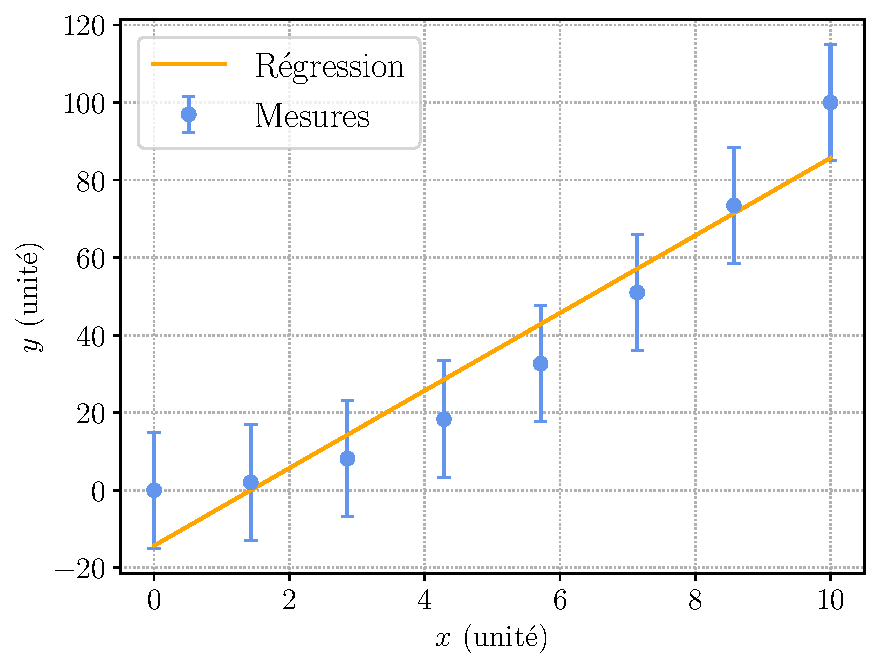
\includegraphics[width=\linewidth, draft=true]{reglin-0}
					\vspace{-15pt}
					\captionof{figure}{Régre$^\circ$ non valide.}
				}{%
					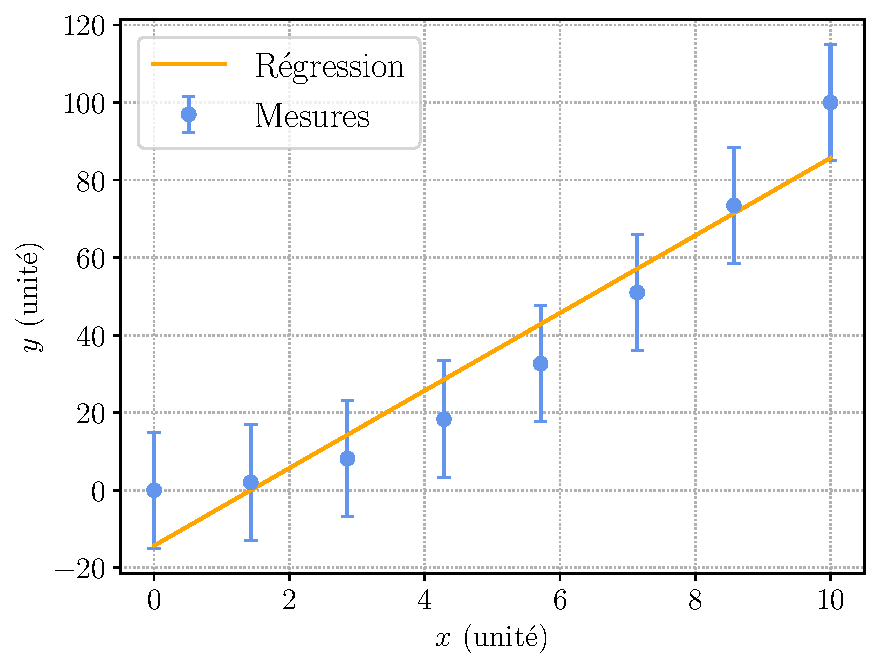
\includegraphics[width=\linewidth]{reglin-0}
					\vspace{-15pt}
					\captionof{figure}{Régre$^\circ$ non valide. \protect \pt{1}}
				}%
			\end{center}
		\end{minipage}
		\hfill
		\begin{minipage}[t]{.48\linewidth}
			\vspace{0pt}
			\begin{center}
				\sswitch{
					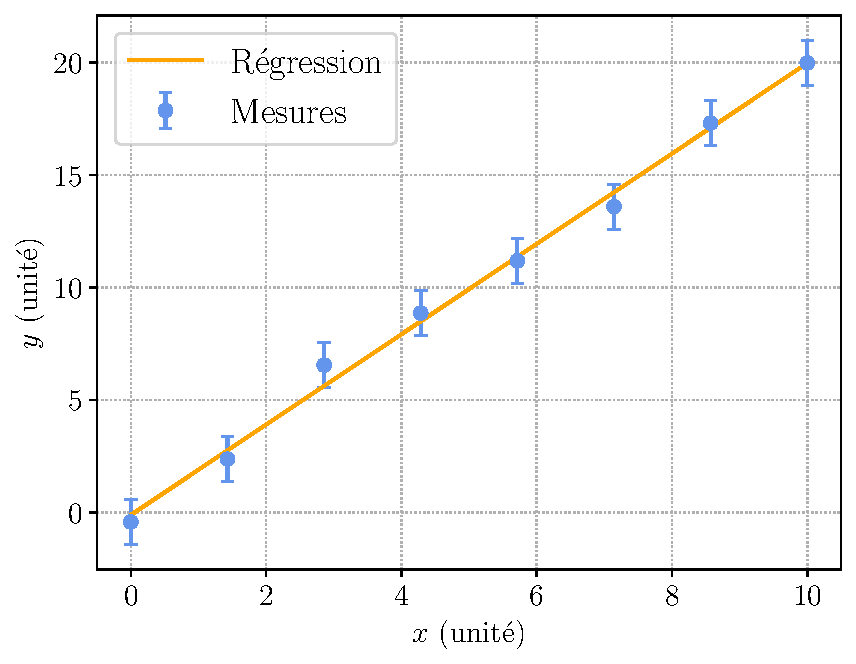
\includegraphics[width=\linewidth, draft=true]{reglin-1}
					\vspace{-15pt}
					\captionof{figure}{Régre$^\circ$ valide.}
				}{%
					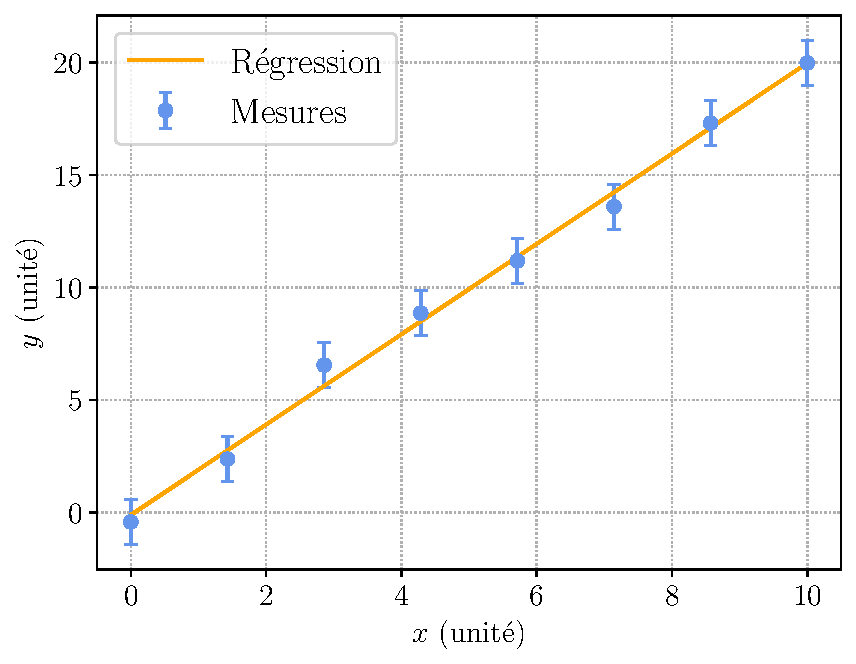
\includegraphics[width=\linewidth]{reglin-1}
					\vspace{-15pt}
					\captionof{figure}{Régre$^\circ$ valide. \protect \pt{1}}
				}%
			\end{center}
		\end{minipage}
		% \vspace*{-20pt}
	\end{isd}
	\item[n]{6}%
	Comment écrire théoriquement un résultat de mesure en TP~? Que doit respecter
	l'écriture de l'incertitude~? Corriger alors la présentation des valeurs
	suivantes.
	% Comment se définit l'incertitude relative~?
	\[
		\lambda = \SI{589.0\pm11}{nm}
		\qquad
		t = \SI{0.473 \pm 0.122}{s}
		\qquad
		V = (14 \pm \num{0.0015})\,\si{mL}
	\]
	\smallbreak
	\noindent
	\begin{isd}[lefthand ratio=.45]
		\psw{%
			Le résultat numérique d'une grandeur $x$ s'écrit~:
			\[
				\boxed{%
					x \stm[-1]{=}
					\left(x\ind{exp} \pm u(x\ind{exp})\right)10^{n} \, \text{unité}
				}%
			\]
		}%
		\vspace{-15pt}
		\tcblower
		\psw{%
			L'incertitude $u(x\ind{exp})$ s'écrit avec 2 chiffres significatifs
			\pt{1}, et
			ces chiffres doivent correspondre aux derniers chiffres de la mesure
			principale. \pt{1}
		}%
		\vspace{-15pt}
	\end{isd}
	\vspace{-15pt}
	\psw{%
		\begin{gather*}
			\beforetext{On trouve}
			\lambda \stm{=} \SI{589\pm11}{nm}
			\qquad
			t \stm{=} \SI{0.47 \pm 0.12}{s}
			\qquad
			V \stm{=} \SI{14.0000 \pm 0.0015}{mL}
		\end{gather*}
		% L'incertitude relative est le pourcentage qu'elle représente par rapport à
		% la mesure~: $\boxed{u_r(x\ind{exp}) \stm{=} \frac{u(x\ind{exp})}{x\ind{exp}}}$.
		\vspace{-15pt}
	}%
	% \vspace*{-20pt}
	% \item[n]{2}%
	% Un laser rouge émet un rayonnement de longueur d'onde dans le vide
	% $\lambda_0 = \SI{633}{nm}$. Déterminer sa longueur d'onde $\lambda$ dans du
	% verre, d'indice optique $n = \num{1.5}$. Sa couleur change-t-elle~?
	% \smallbreak
	% \begin{isd}[lefthand ratio=.35]
	% 	\psw{%
	% 		On a
	% 		\begin{gather*}
	% 			\boxed{\lambda = \frac{\lambda_0}{n}}
	% 			\qav
	% 			\left\{
	% 			\begin{array}{rcl}
	% 				\lambda_0 & = & \SI{633}{nm}
	% 				\\
	% 				n         & = & \num{1.5}
	% 			\end{array}
	% 			\right.\\
	% 			\mathrm{A.N.~:}\enskip
	% 			\xul{
	% 				\lambda = \SI{422}{nm}
	% 			}%
	% 		\end{gather*}
	% 	}%
	% 	\vspace*{-20pt}
	% 	\tcblower
	% 	\psw{%
	% 		Cependant, \textbf{sa couleur ne change pas} puis qu'\xul{une onde est
	% 			caracétrisée par sa fréquence}, qui ne change pas.
	% 	}%
	% 	\vspace*{-20pt}
	% \end{isd}
	\item[n]{1.5}%
	Citer le nom des trois propriétés d'un rayon lumineux.
	\psw{%
		\begin{enumerate}
			\item Propagation rectiligne dans un milieu TLHI~;
			\item Indépendance des rayons lumineux,
			\item Retour inverse dans un milieu TLI.
		\end{enumerate}
	}%

	\item[n]{+2}%
	Explain in a few words what the pigeonhole principle is. Give one example of
	what it can prove.
	\smallbreak
	\psw{%
		The pigeonhole principle states that if you have more items than
		containers, then at least one container has more than one item. It can be
		used to prove that the cardinality of $\Rb$ is bigger than the cardinality
		of $\Nb$.
	}%
\end{enumerate}

\ifstudent{
	\begin{tikzpicture}[remember picture, overlay]
		\node[anchor=north west, align=left]
		at ([shift={(1.4cm,0)}]current page.north west)
		{\\[5pt]\Large\bfseries Nom~:\\[10pt]\Large\bfseries Prénom~:};
		\node[anchor=north east, align=right]
		at ([shift={(-1.5cm,-17pt)}]current page.north east)
		{\Large\bfseries Note~:\hspace{1cm}/20};
	\end{tikzpicture}
}
\end{document}
